\documentclass[a4paper,12pt]{report}

\usepackage[utf8x]{inputenc}
\usepackage[T2A]{fontenc}
\usepackage[english, russian]{babel}

% Опционно, требует  apt-get install scalable-cyrfonts.*
% и удаления одной строчки в cyrtimes.sty
% Сточку не удалять!
% \usepackage{cyrtimes}

% Картнки и tikz
\usepackage{graphicx}
\usepackage{tikz}
\usetikzlibrary{snakes,arrows,shapes}


% Увы, поля придётся уменьшить из-за листингов.
\topmargin -1cm
\oddsidemargin -0.5cm
\evensidemargin -0.5cm
\textwidth 17cm
\textheight 24cm

\sloppy



% Оглавление в PDF
\usepackage[
bookmarks=true,
colorlinks=true, linkcolor=black, anchorcolor=black, citecolor=black, menucolor=black,filecolor=black, urlcolor=black,
unicode=true
]{hyperref}

% Для исходного кода в тексте
% \newcommand{\Code}[1]{\texttt{#1}}

% Некоторая русификация.
% \usepackage{misccorr} % Oh shi^W^W, оно не работает с report.
\usepackage{indentfirst}
\renewcommand{\labelitemi}{\normalfont\bfseries{--}}

% На дворе XXI век, но пакет listings всё ещё не пашет с русскими комментариями!

% Пакет listings для простой вставки исходников
% \usepackage{listings}
% Параметры оформления
% \lstset{
% showspaces=false,
% showtabs=false,
% frame=single,
% tabsize=4,
% basicstyle=\ttfamily,
% identifierstyle=\ttfamily,
% commentstyle=\itshape,
% stringstyle=\ttfamily,
% keywordstyle=\ttfamily,
% breaklines=true
% }
% Русский в комментариях.
% \lstset{escapebegin=\begin{cyr},escapeend=\end{cyr}}



% А это взято из файла, сгенерённого doxygen
\usepackage{calc}
\usepackage{array}
\newenvironment{Code}
{\footnotesize}
{\normalsize}
\newcommand{\doxyref}[3]{\textbf{#1} (\textnormal{#2}\,\pageref{#3})}
\newenvironment{DocInclude}
{\footnotesize}
{\normalsize}
\newenvironment{VerbInclude}
{\footnotesize}
{\normalsize}
\newenvironment{Image}
{\begin{figure}[H]}
{\end{figure}}
\newenvironment{ImageNoCaption}{}{}
\newenvironment{CompactList}
{\begin{list}{}{
  \setlength{\leftmargin}{0.5cm}
  \setlength{\itemsep}{0pt}
  \setlength{\parsep}{0pt}
  \setlength{\topsep}{0pt}
  \renewcommand{\makelabel}{\hfill}}}
{\end{list}}
\newenvironment{CompactItemize}
{
  \begin{itemize}
  \setlength{\itemsep}{-3pt}
  \setlength{\parsep}{0pt}
  \setlength{\topsep}{0pt}
  \setlength{\partopsep}{0pt}
}
{\end{itemize}}
\newcommand{\PBS}[1]{\let\temp=\\#1\let\\=\temp}
\newlength{\tmplength}
\newenvironment{TabularC}[1]
{
\setlength{\tmplength}
     {\linewidth/(#1)-\tabcolsep*2-\arrayrulewidth*(#1+1)/(#1)}
      \par\begin{tabular*}{\linewidth}
             {*{#1}{|>{\PBS\raggedright\hspace{0pt}}p{\the\tmplength}}|}
}
{\end{tabular*}\par}
\newcommand{\entrylabel}[1]{
   {\parbox[b]{\labelwidth-4pt}{\makebox[0pt][l]{\textbf{#1}}\vspace{1.5\baselineskip}}}}
\newenvironment{Desc}
{\begin{list}{}
  {
    \settowidth{\labelwidth}{40pt}
    \setlength{\leftmargin}{\labelwidth}
    \setlength{\parsep}{0pt}
    \setlength{\itemsep}{-4pt}
    \renewcommand{\makelabel}{\entrylabel}
  }
}
{\end{list}}
\newenvironment{Indent}
  {\begin{list}{}{\setlength{\leftmargin}{0.5cm}}
      \item[]\ignorespaces}
  {\unskip\end{list}}



\title{Отчёт по лабораторной работе \textnumero 1}
\author{(Ф.~И.~О)}

\begin{document}

\maketitle

\tableofcontents

\addcontentsline{toc}{chapter}{Введение}
\chapter*{Введение}

Два предложения о содержании отчёта. Для нового абзаца в исходном тексте должна быть пустая строка.

Это~-- шаблон отчёта (вот как оформляется длинное тире, перед котрым идёт неразрывный пробел).


Здесь должно быть вербальное задание.

А вот так оформляются списки:
\begin{itemize}
\item элемент списка;
\item последний элемент списка.
\end{itemize}

Нумерованный список выглядит следующим образом.
\begin{enumerate}
\item Первый элемент.
\item Второй элемент.
\end{enumerate}

% \chapter{Аналитический раздел}

\chapter{Конструкторский раздел}

\section{Конечный автомат состояний сервера}

Рис.~\ref{fig:fsm} нагенерил самодельный \textit{fsm2dot} из \textit{autogen} и \textit{dot2tex} на пару \textit{dot}. Никто не мешает изменить параметры типа \textit{rankdir} прямо в \textit{fsm2dot}, если он будет лучше смотреться, например, сверху-вниз.

\begin{figure}
\centering
% \includegraphics[width=\textwidth]{include/server_def_dot.pdf}
\caption{Состояния сервера}
\label{fig:fsm}
\end{figure}

\section{Синтаксис команд протокола}

\begin{description}
\item[Команда выхода из сеанса]
% \input{include/re_cmd_quit_re.tex}
\item[Команда передачи имени пользователя]
% \input{include/re_cmd_user_re.tex}
\end{description}

Для грамматики можно использовать вставку из файла и оформление \textbackslash{}begin\{verbatim\} и \textbackslash{}end\{verbatim\} или пакет \textit{listings}\footnote{На дворе XXI век, но пакет \textit{listings} всё ещё не пашет с русскими комментариями без бубна, и лично я его пока не победил.}.

Для примера воспользуемся автоматической вставкой файла описания параметров программы (не забудьте перенести это в технологический раздел) через утилитку \textit{src2tex}.

% \input{include/checkoptn.def.tex}
% \lstset{language=C}
% \lstinputlisting{../src/checkoptn.def}

\chapter{Технологический раздел}

Нужно отметьть, что символ <<\_>> необходимо оформлять как <<\textbackslash\_>>.

\section{Сборка программы}

Сборка программы описана в файле \textit{Makefile} системы сборки \textit{make}. Рис.~\ref{fig:make} нагенерили самодельные \textit{makesimple} и \textit{makefile2dot}, а также \textit{dot2tex} и \textit{dot}.

\begin{figure}
\centering
% \includegraphics[width=\textwidth]{include/Makefile_1_dot.pdf}
\caption{Сборка программы}
\label{fig:make}
\end{figure}

Отмечу, что за исключения целей типа \textit{all}, \textit{install}, \textit{clean}, \textit{tests}, все имена целей в файле систем сборки \textit{make} обычно совпадают с именами файлов (такой вот низкоуровневый инструмент). То есть вместо цели \textit{lexer} следует использовать цель \textit{src/lexer.c}.

\section{Основные функции программы}

Весь это раздел сгеренерировал doxygen из части комментированных исходников программы. В файле конфигурации \textbf{doxyggen.cfg} был отключён параметр \textbf{HAVE\_DOT}, поскольку для рисования графов вызовов используется \textit{cflow}.

% \input{include/files}

% \input{include/server-state_8h.tex}
% \input{include/server-state_8c.tex}
% \input{include/server-re_8h.tex}
% \input{include/server-cmd_8h.tex}
% \input{include/server-cmd_8c.tex}
% \input{include/server-parse_8h.tex}
% \input{include/server-parse_8c.tex}
% \input{include/server-run_8h.tex}
% \input{include/server-run_8c.tex}
% \input{include/server_8c.tex}


\section{Графы вызова функций}

Поскольку функций много, графы вызовов разбиты на два рисунка. На рис.~\ref{fig:ccflow01} показаны основные функции, на рис.~\ref{fig:scflow01}~-- функции обработки команд. Файл \textbf{cflow.ignore} содержит список функций (точнее, шабловнов поиска), использыемых программой \textit{grep} для удаления малоинтересных стандартных функций\footnote{Функции по работе с сокетами, ipc и привилегиями к малоинтересным ни в коем случае не относятся.}.

\begin{figure}
\centering
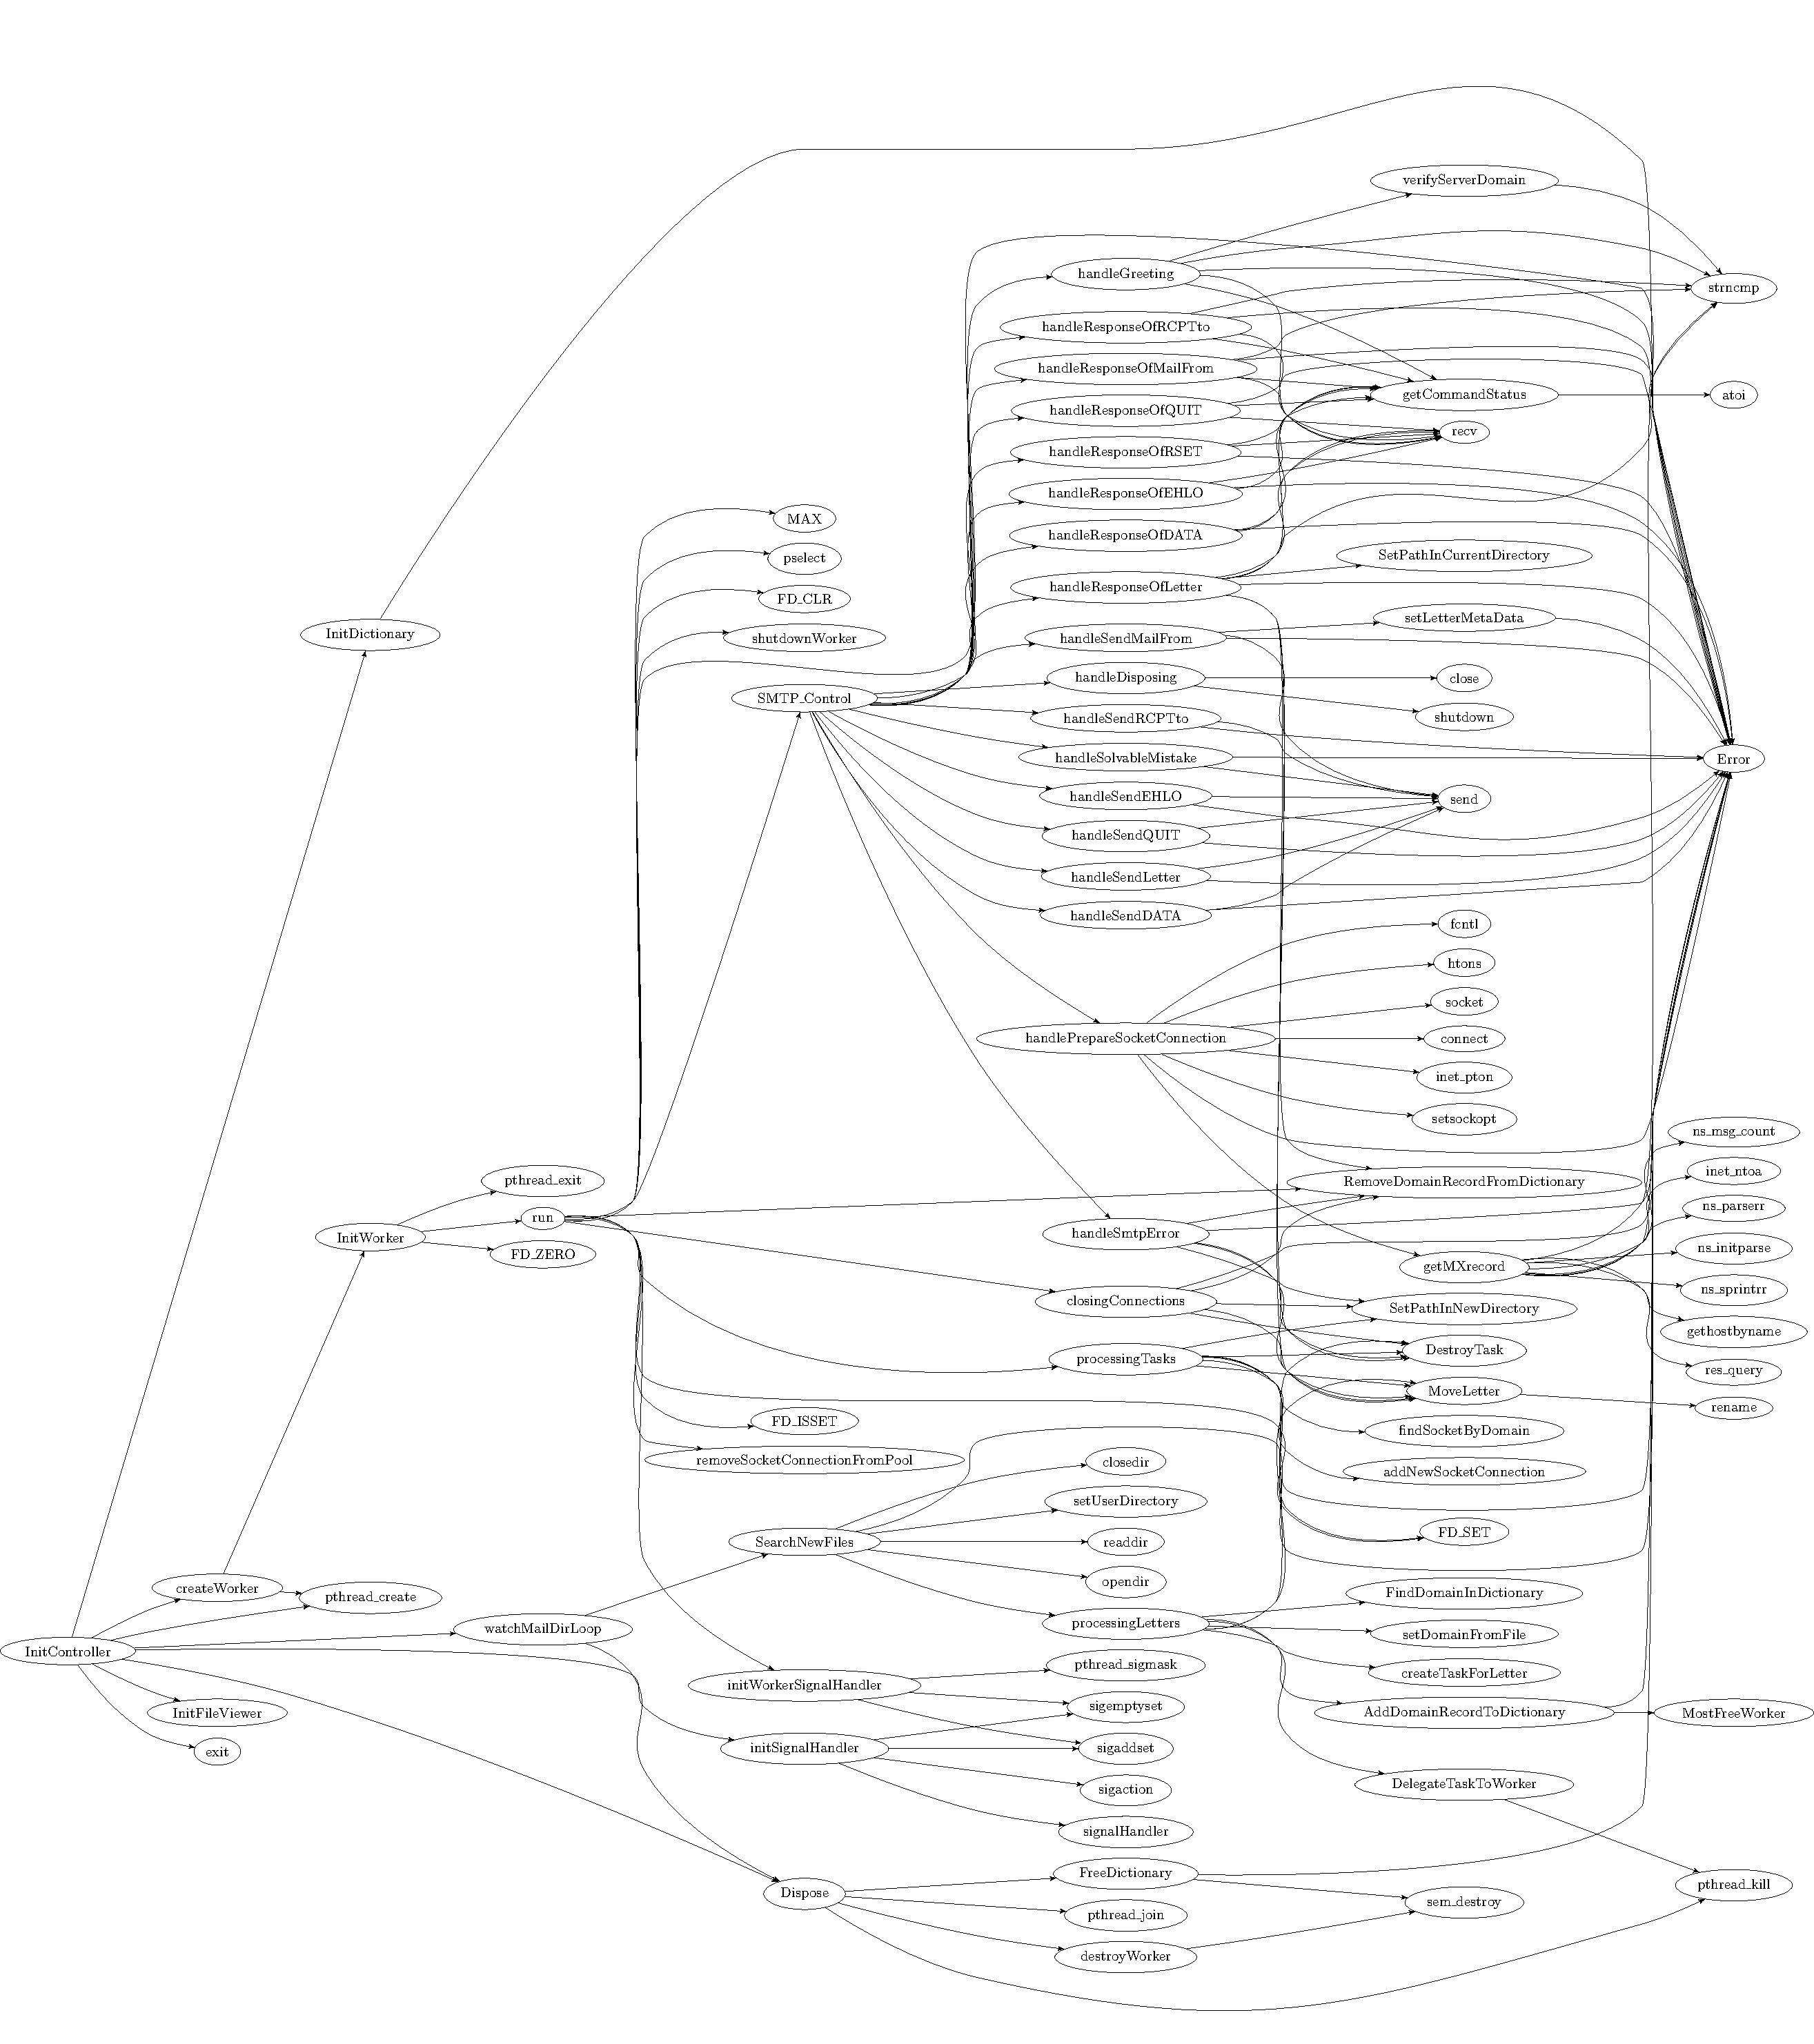
\includegraphics[width=\textwidth]{include/ccflow01_dot.pdf}
\caption{Граф вызовов, основные функции}
\label{fig:ccflow01}
\end{figure}

\begin{figure}
\centering
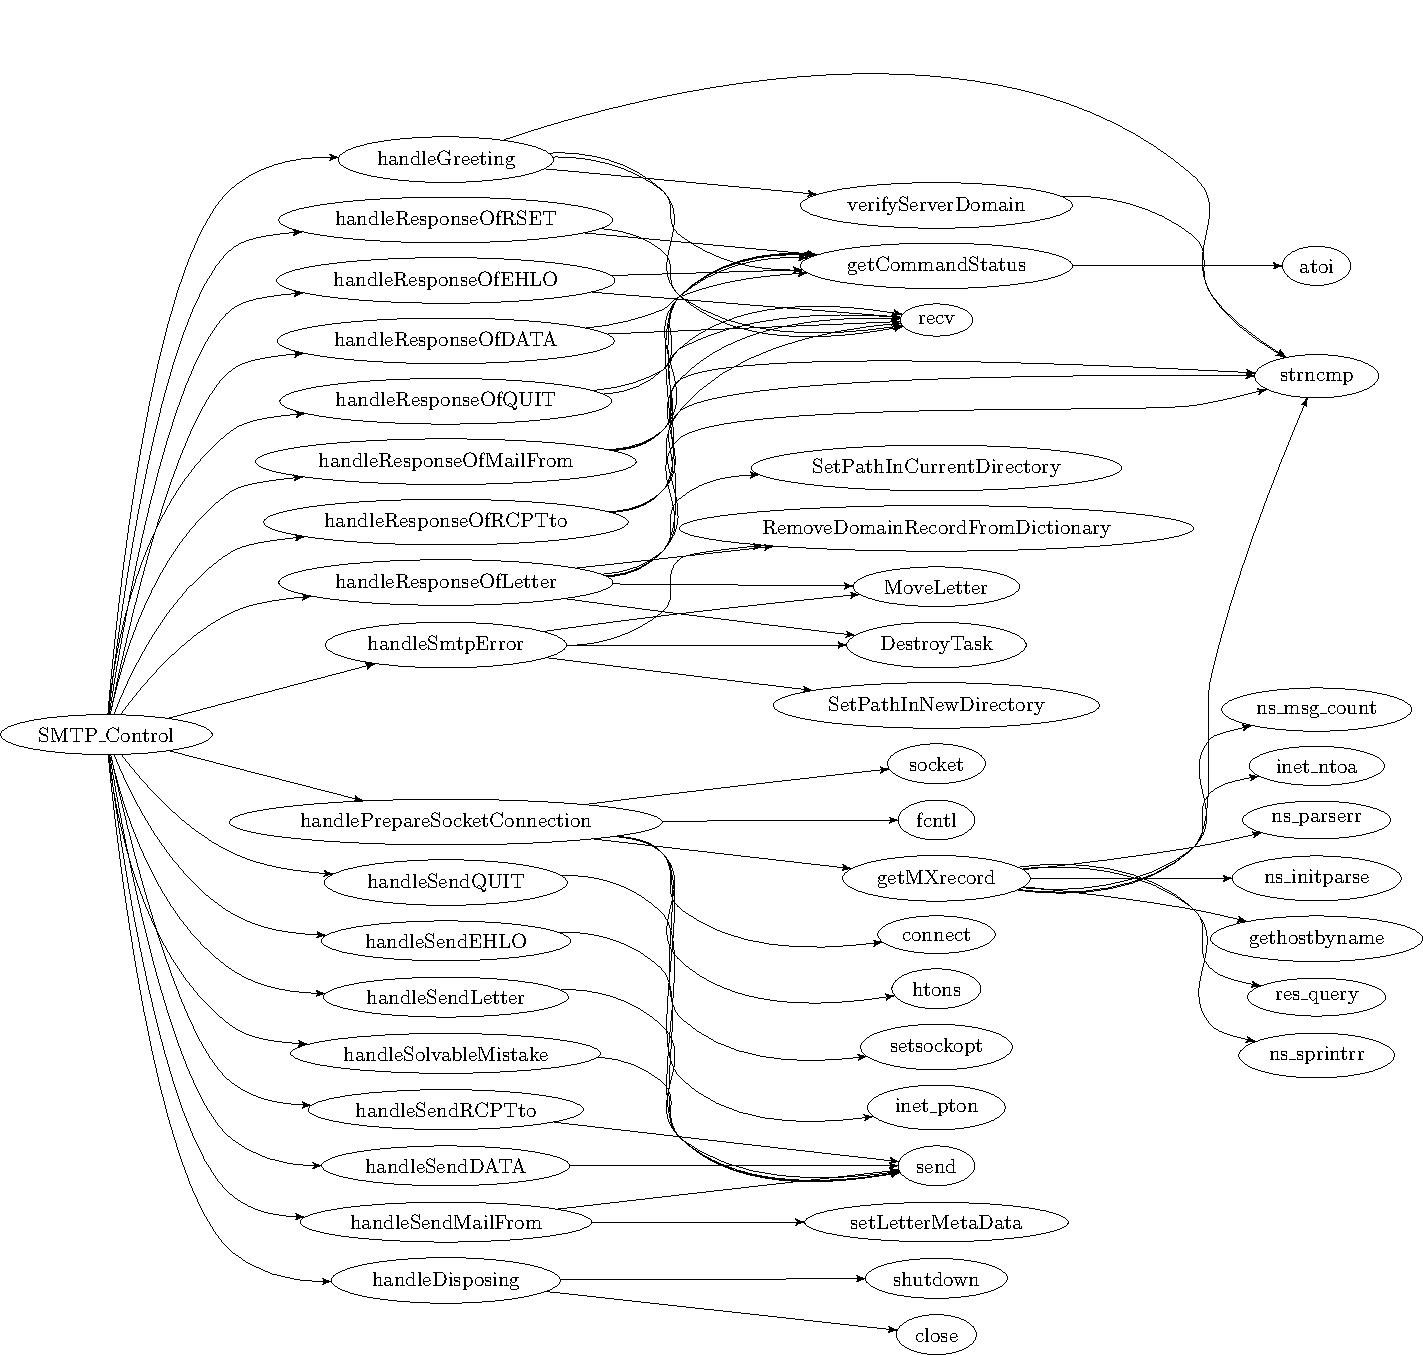
\includegraphics[width=\textwidth]{include/ccflow02_dot.pdf}
\caption{Граф вызовов, основные функции}
\label{fig:ccflow02}
\end{figure}

\begin{figure}
\centering
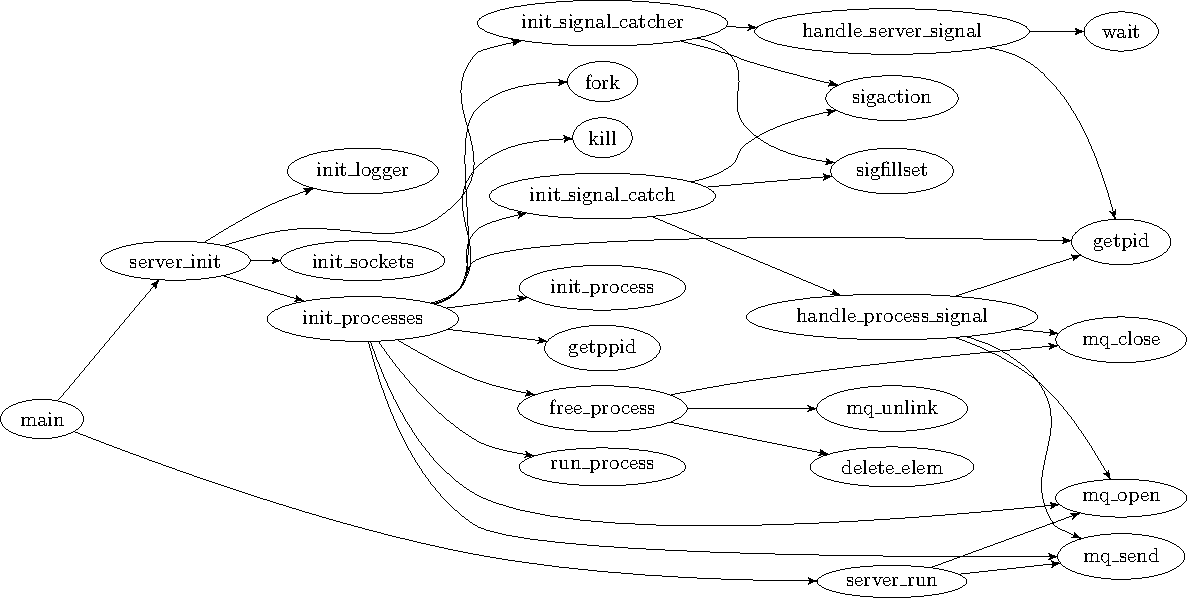
\includegraphics[width=\textwidth]{include/scflow01_dot.pdf}
\caption{Граф вызовов, функции обработки команд}
\label{fig:scflow01}
\end{figure}

\begin{figure}
\centering
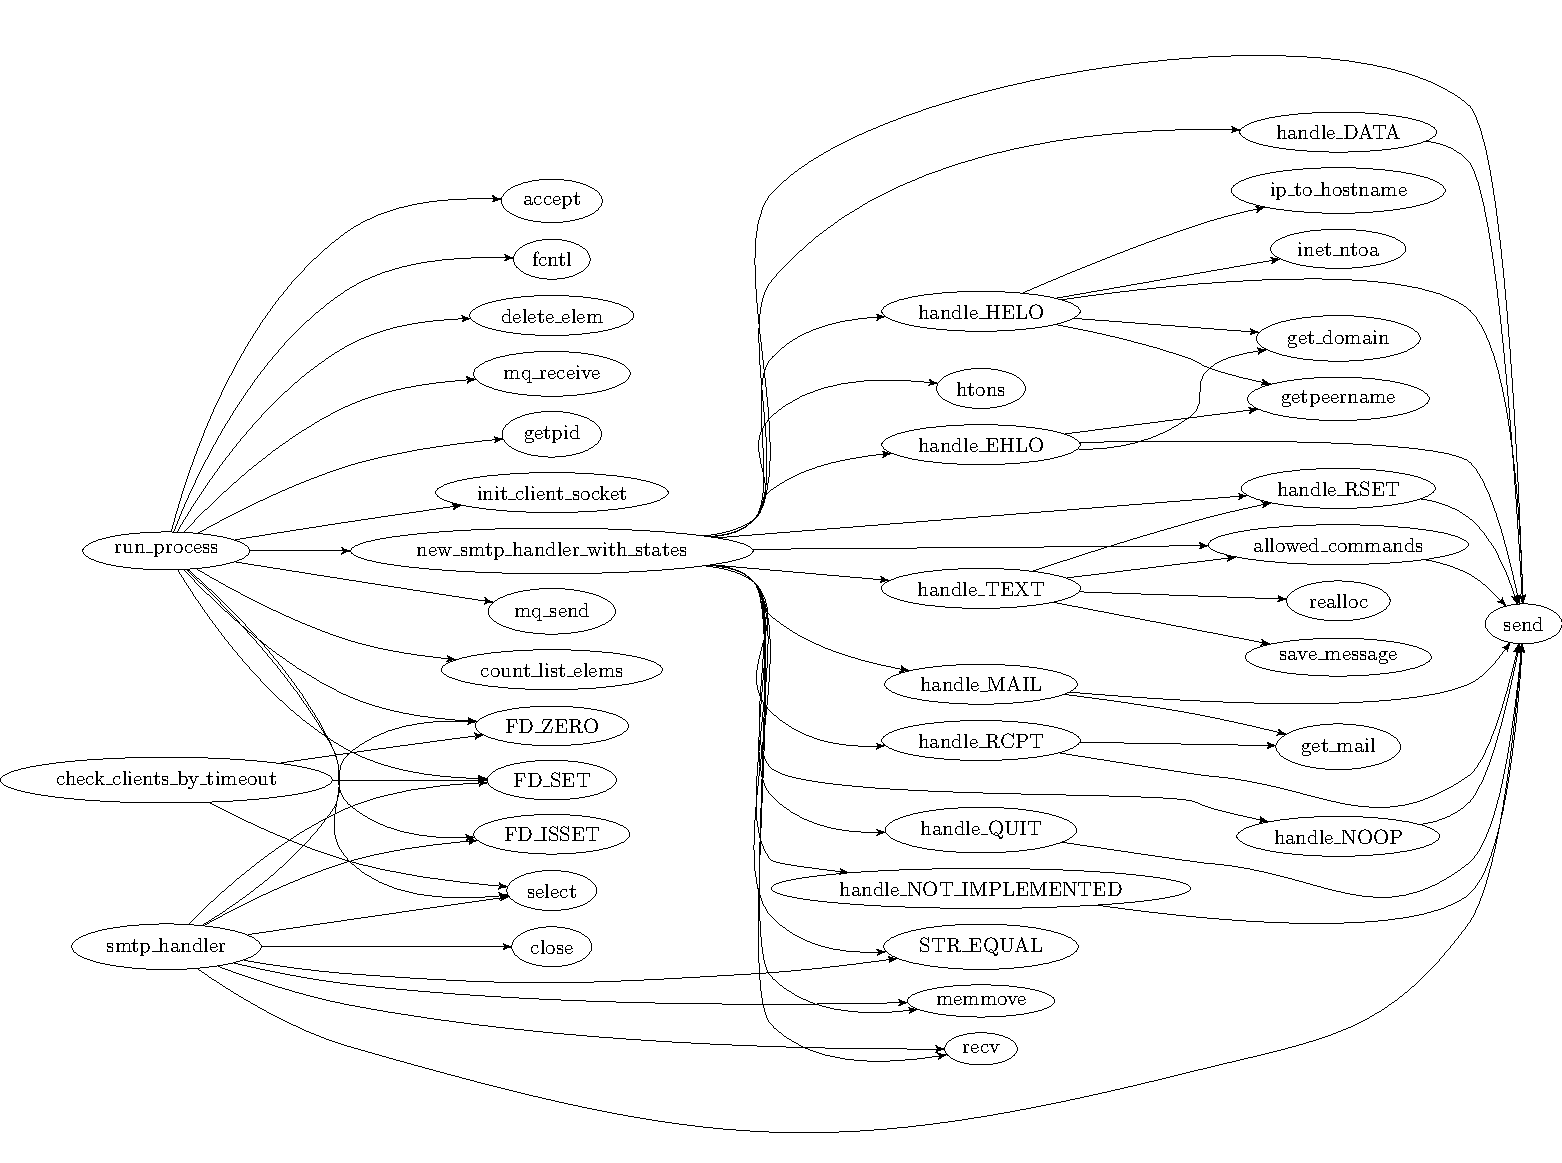
\includegraphics[width=\textwidth]{include/scflow02_dot.pdf}
\caption{Граф вызовов, функции обработки команд}
\label{fig:scflow01}
\end{figure}

Графы созданы с помощью \textit{cflow}, \textit{cflow2dot}, \textit{dot}.

\addcontentsline{toc}{chapter}{Выводы}
\chapter*{Выводы}

Что вы сделали и поняли.


\end{document}
